\begin{figure}[t!]
    \centering
    % \begin{tabular}[c]{ccc}
    % \begin{subfigure}[c]{0.31\textwidth}
    %     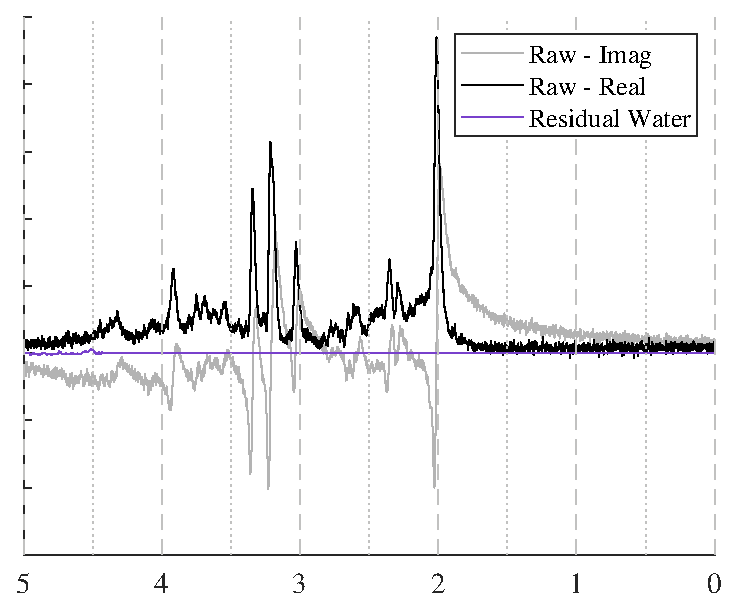
\includegraphics[width=0.93\textwidth]{images/samples_by_artifact/30ms_artifact_samples_ecc_1.eps}
    %     \caption{$A=1.0$ Hz, $t_c=0.15$ s}
    %     \vspace{3pt}
    % \end{subfigure}&
    % \begin{subfigure}[c]{0.31\textwidth}
    %     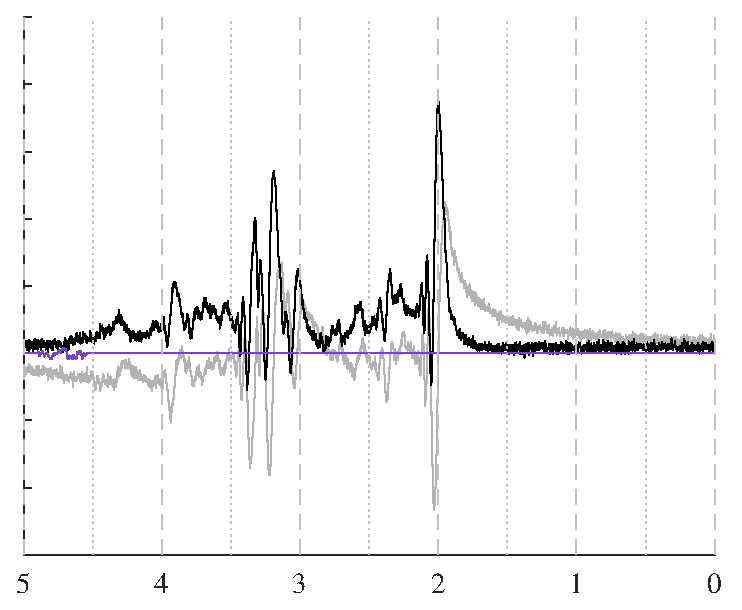
\includegraphics[width=0.93\textwidth]{images/samples_by_artifact/30ms_artifact_samples_ecc_2.eps}
    %     \caption{$A=5.5$ Hz, $t_c=0.15$ s}
    %     \vspace{3pt}
    % \end{subfigure}&
    % \begin{subfigure}[c]{0.31\textwidth}
    %     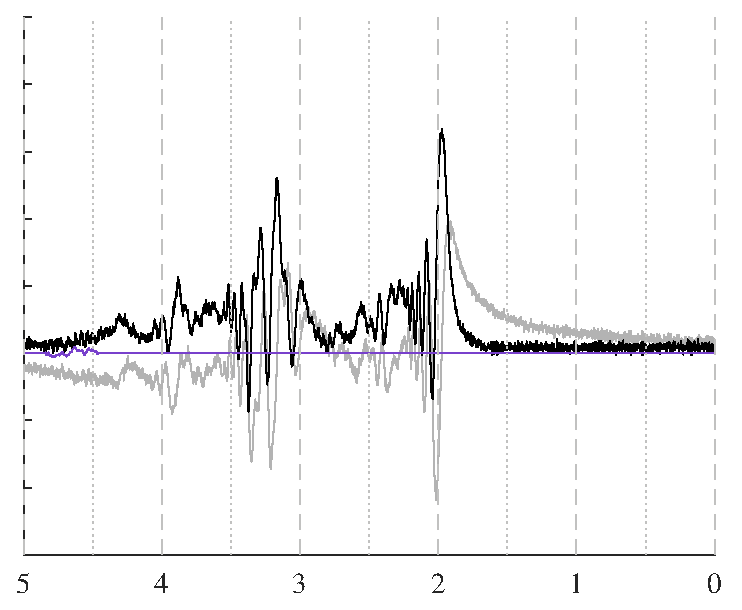
\includegraphics[width=0.93\textwidth]{images/samples_by_artifact/30ms_artifact_samples_ecc_3.eps}
    %     \caption{$A=10.0$ Hz, $t_c=0.15$ s}
    %     \vspace{3pt}
    % \end{subfigure}\\
    % \begin{subfigure}[c]{0.31\textwidth}
    %     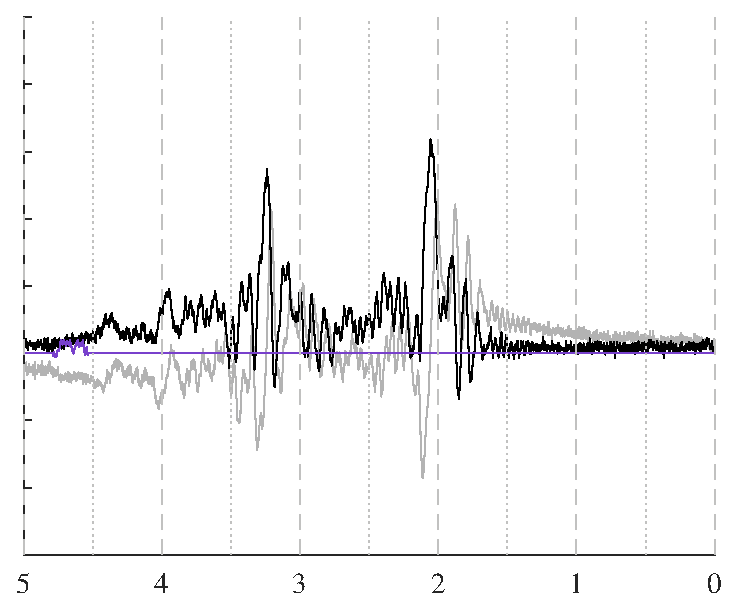
\includegraphics[width=0.93\textwidth]{images/samples_by_artifact/30ms_artifact_samples_ecc_4.eps}
    %     \caption{$A=5.0$ Hz, $t_c=0.02$ s}
    %     % \vspace{3pt}
    % \end{subfigure}&
    % \begin{subfigure}[c]{0.31\textwidth}
    %     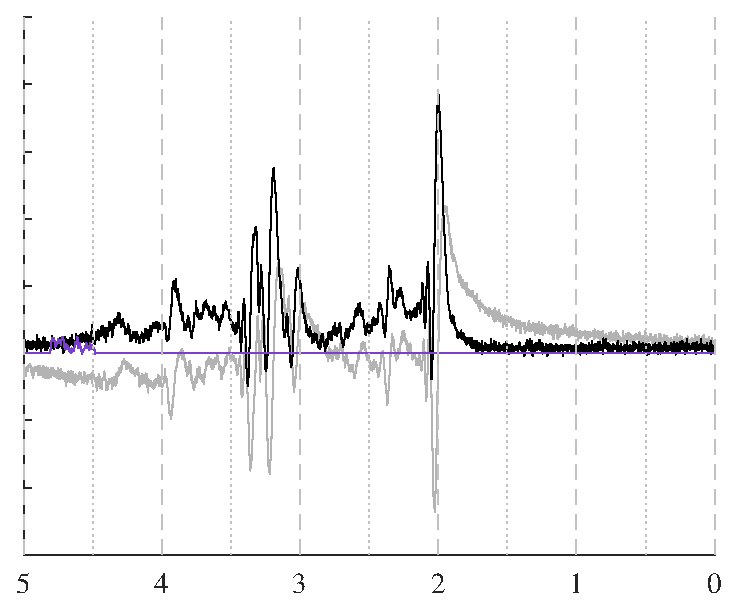
\includegraphics[width=0.93\textwidth]{images/samples_by_artifact/30ms_artifact_samples_ecc_5.eps}
    %     \caption{$A=5.0$ Hz, $t_c=0.16$ s}
    %     % \vspace{3pt}
    % \end{subfigure}&%
    % \begin{subfigure}[c]{0.31\textwidth}
    %     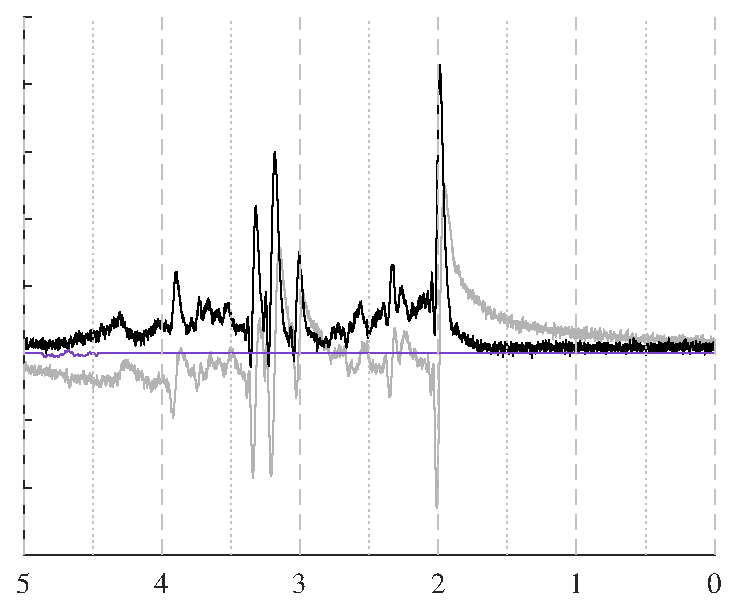
\includegraphics[width=0.93\textwidth]{images/samples_by_artifact/30ms_artifact_samples_ecc_6.eps}
    %     \caption{$A=5.0$ Hz, $t_c=0.30$ s}
    %     % \vspace{3pt}
    % \end{subfigure}\\
    % \end{tabular}
    \includegraphics[width=0.95\textwidth,keepaspectratio]{images/compiled_figures/MRS_Sim_Figure_15_ECC_samples.png}
    \caption{Eddy currents are simulated with two variables: an amplitude, A, and a time constant, $t_c$. In the top row, $t_c$ is fixed to 0.15 seconds and the amplitudes are set to 1Hz, 5.5Hz, and 10Hz. In the bottom row, the amplitude is fixed to 5Hz and the time constants are set to 0.02 sec, 0.16 sec, and 0.30 sec. The values listed correspond to the plots from left to right.}
    \label{fig:30ms samples ecc}
\end{figure}

